\newpage
\section{Anhang}

\subsection{Versuchsaufbauten}
\begin{figure}[H]
    \centering
    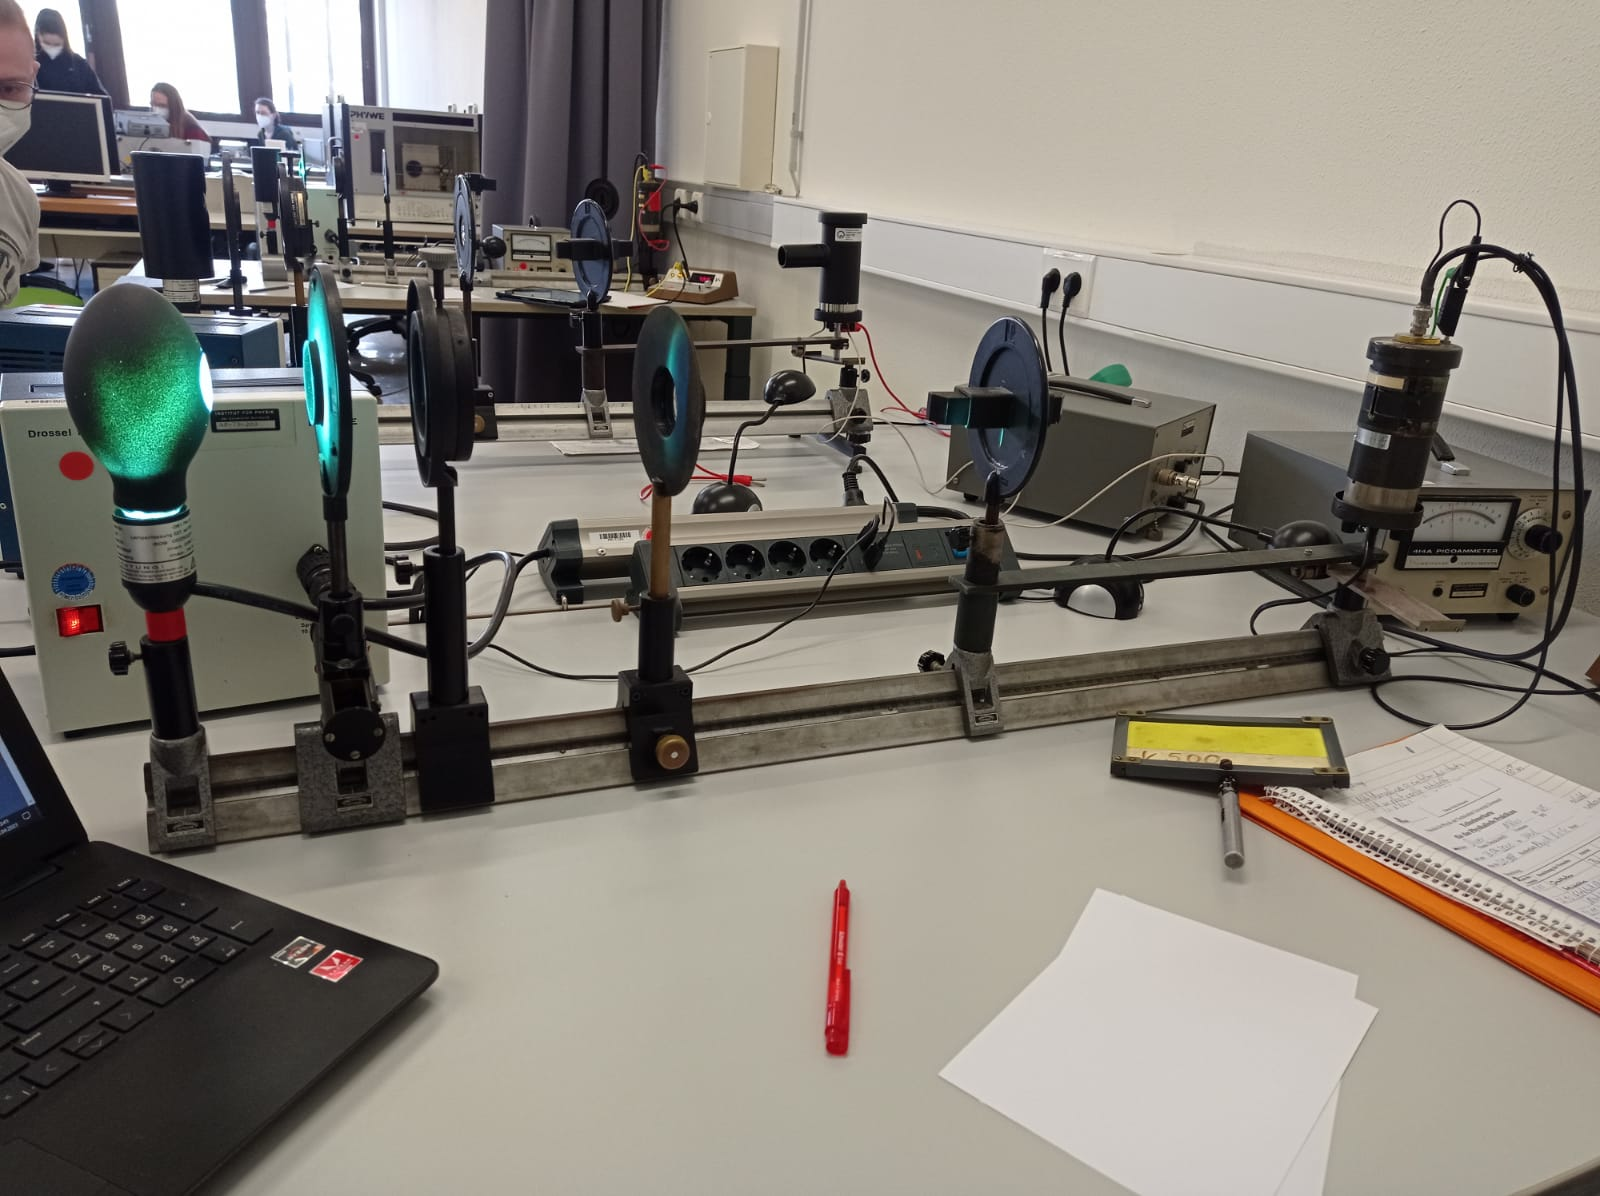
\includegraphics[width=0.63\textwidth]{latex/images/Aufbau_Photoeffekt.jpeg}
    \caption{Ein Foto des Aufbaus um den Photoeffekt zu untersuchen.}
    \label{img:aufbau}
\end{figure}

\subsection{Daten}
\begin{figure}[H]
    \centering
    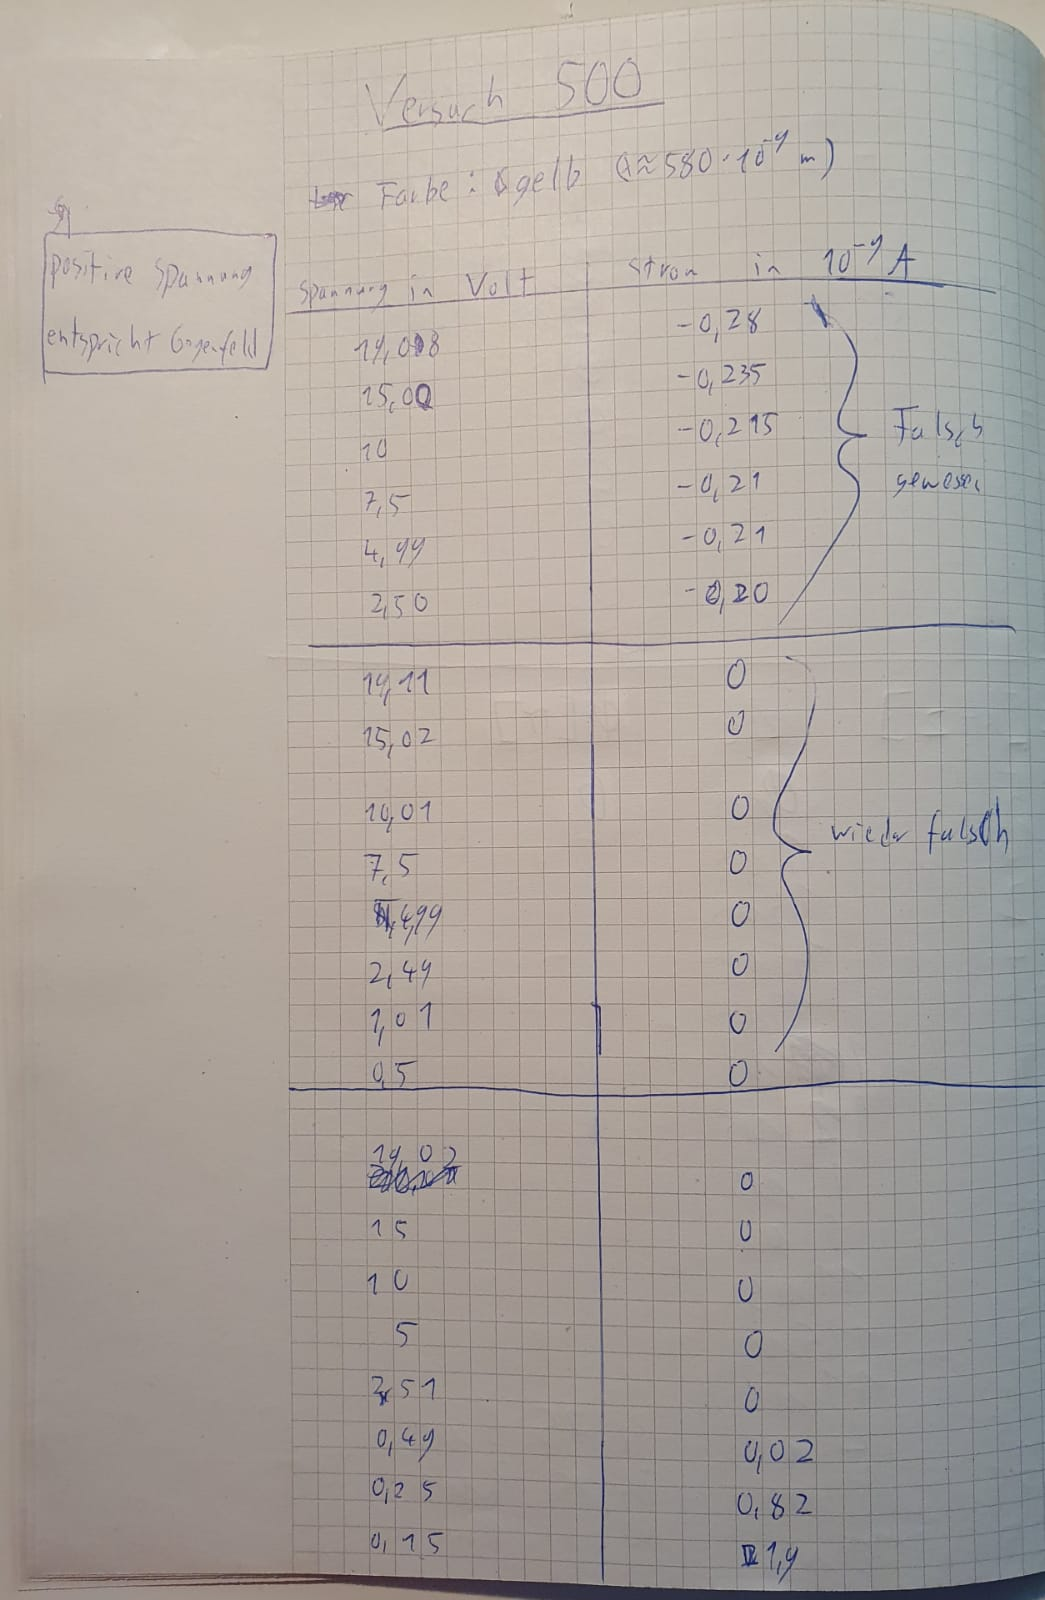
\includegraphics[width=0.63\textwidth]{latex/images/D1.jpeg}
    \caption{Ein Foto der Messdaten.}
    \label{img:Daten1}
\end{figure}
\begin{figure}[H]
    \centering
    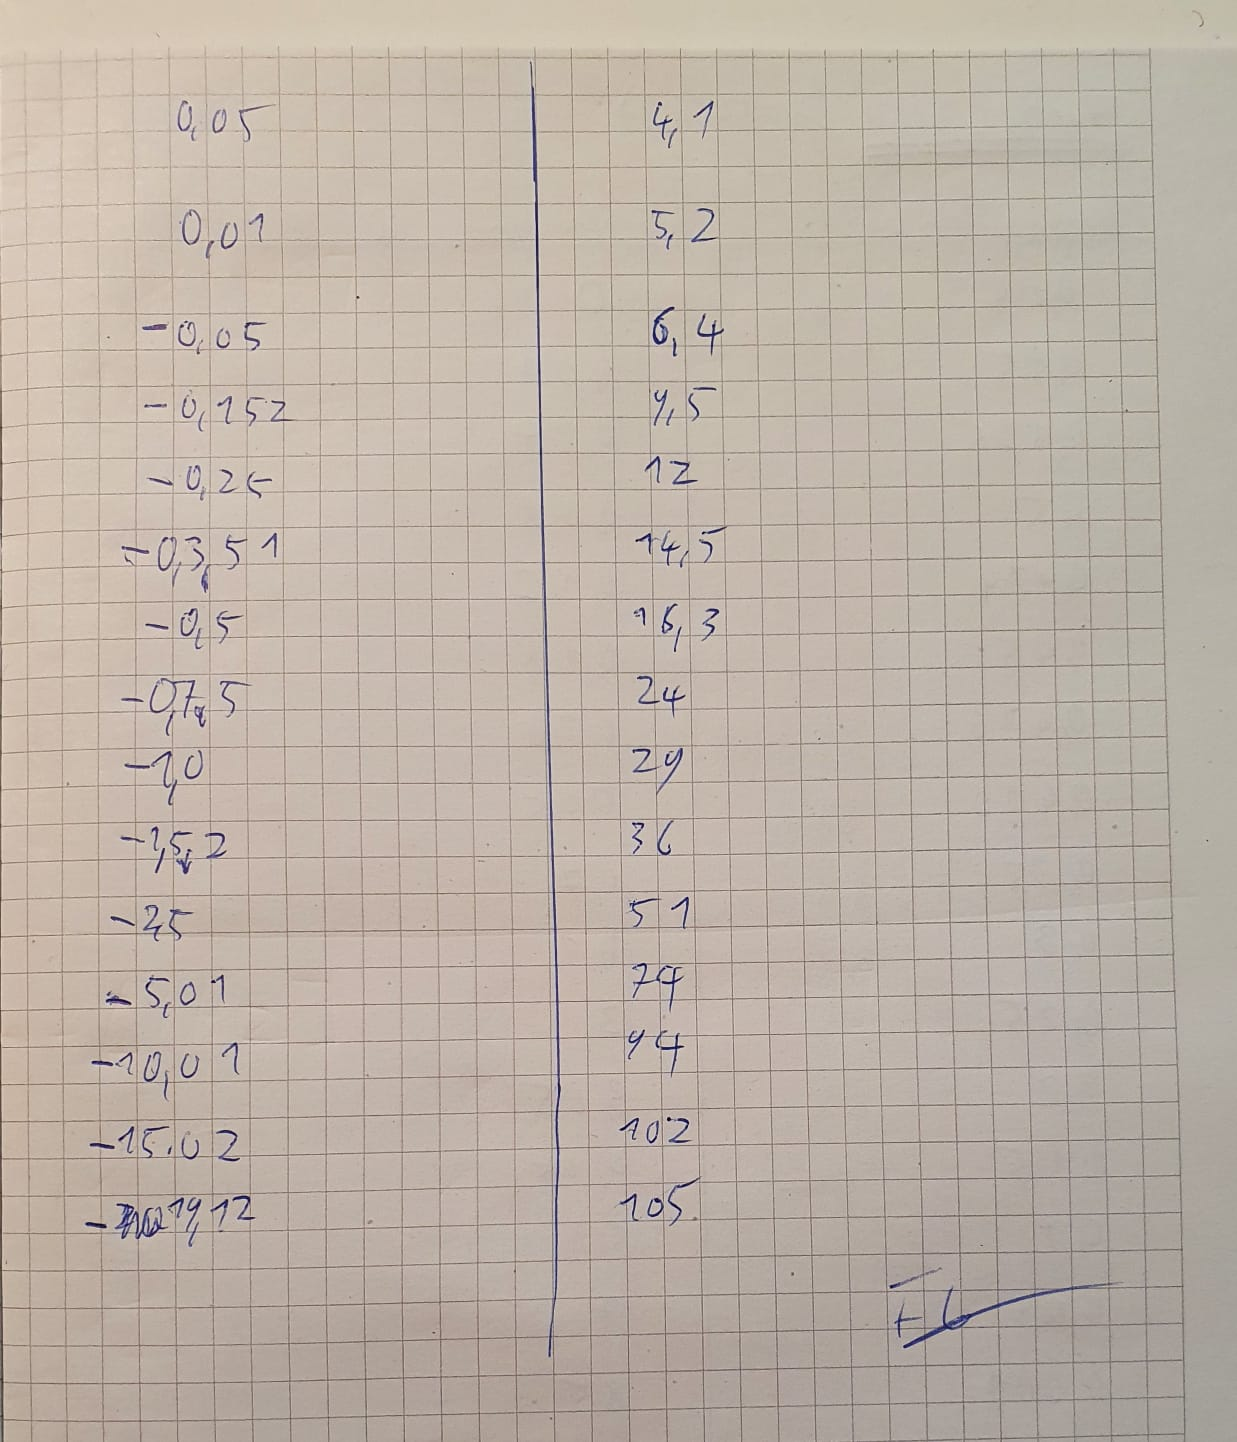
\includegraphics[width=0.63\textwidth]{latex/images/D2.jpeg}
    \caption{Ein Foto der Messdaten.}
    \label{img:Daten2}
\end{figure}
\begin{figure}[H]
    \centering
    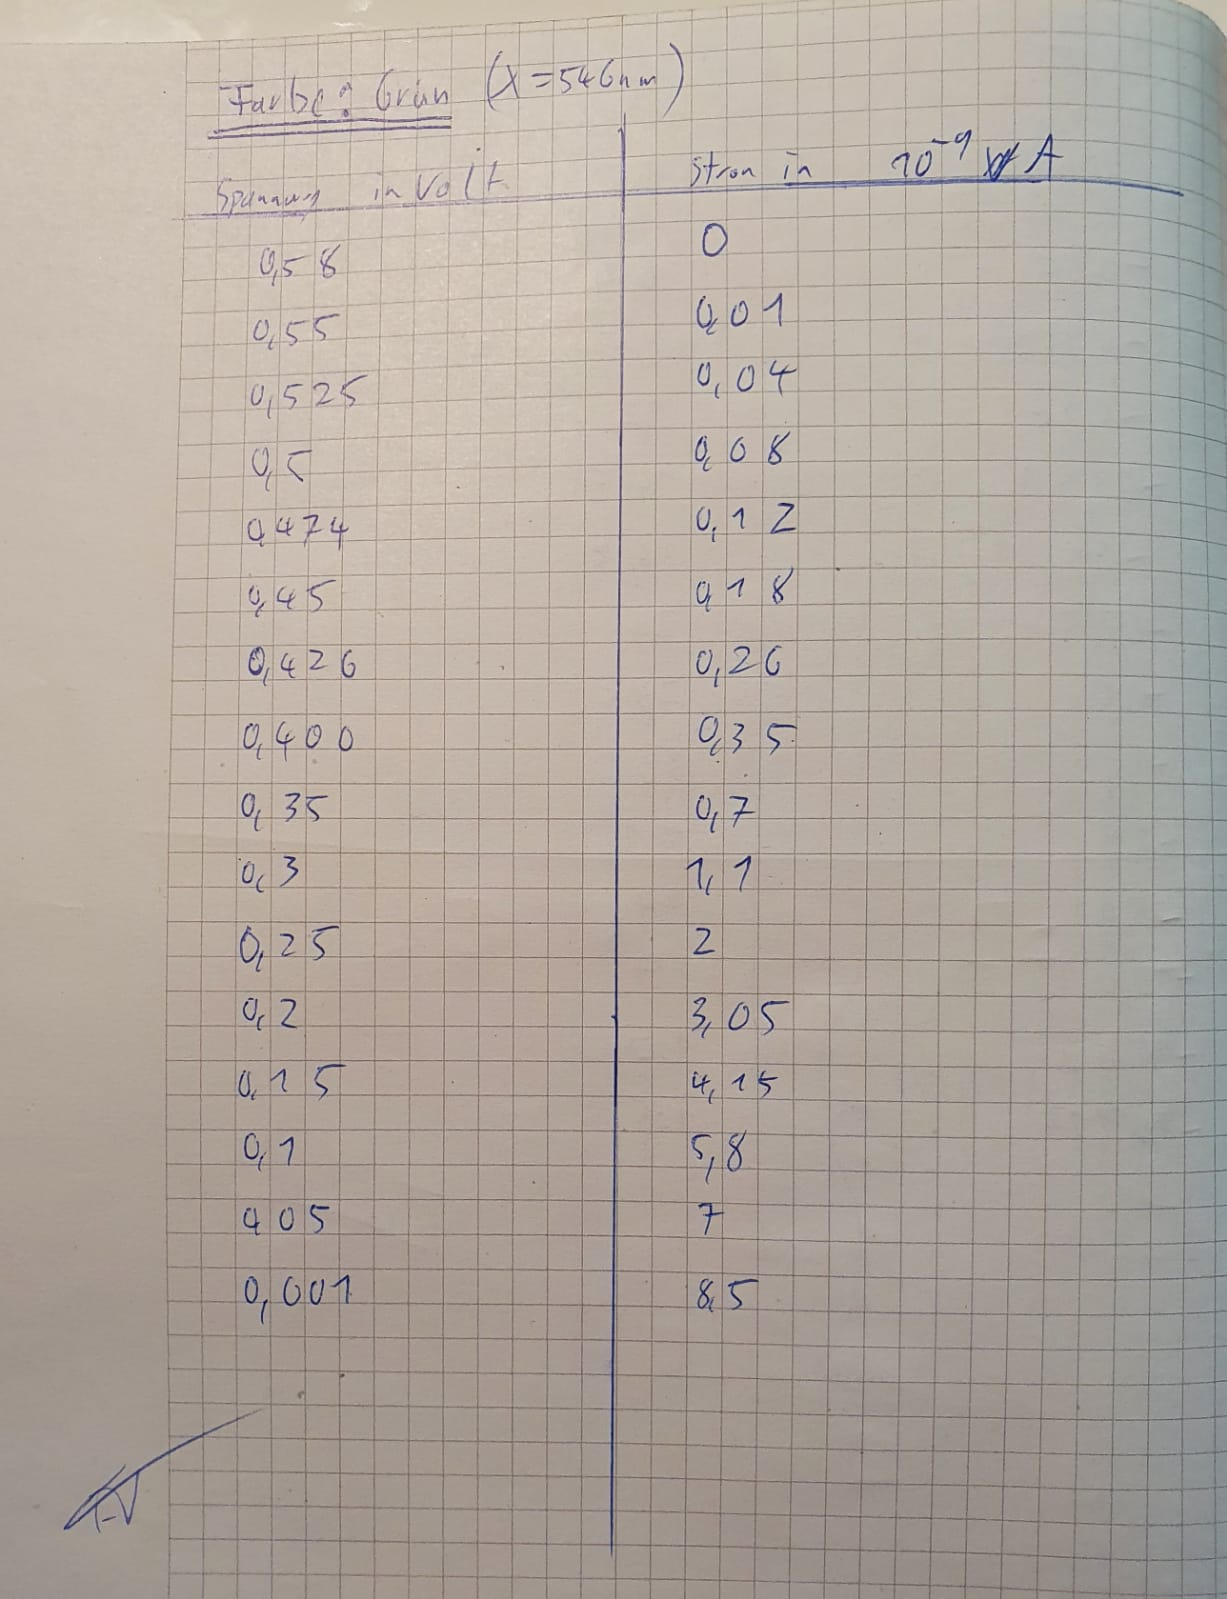
\includegraphics[width=0.63\textwidth]{latex/images/D3.jpeg}
    \caption{Ein Foto der Messdaten.}
    \label{img:Daten3}
\end{figure}
\begin{figure}[H]
    \centering
    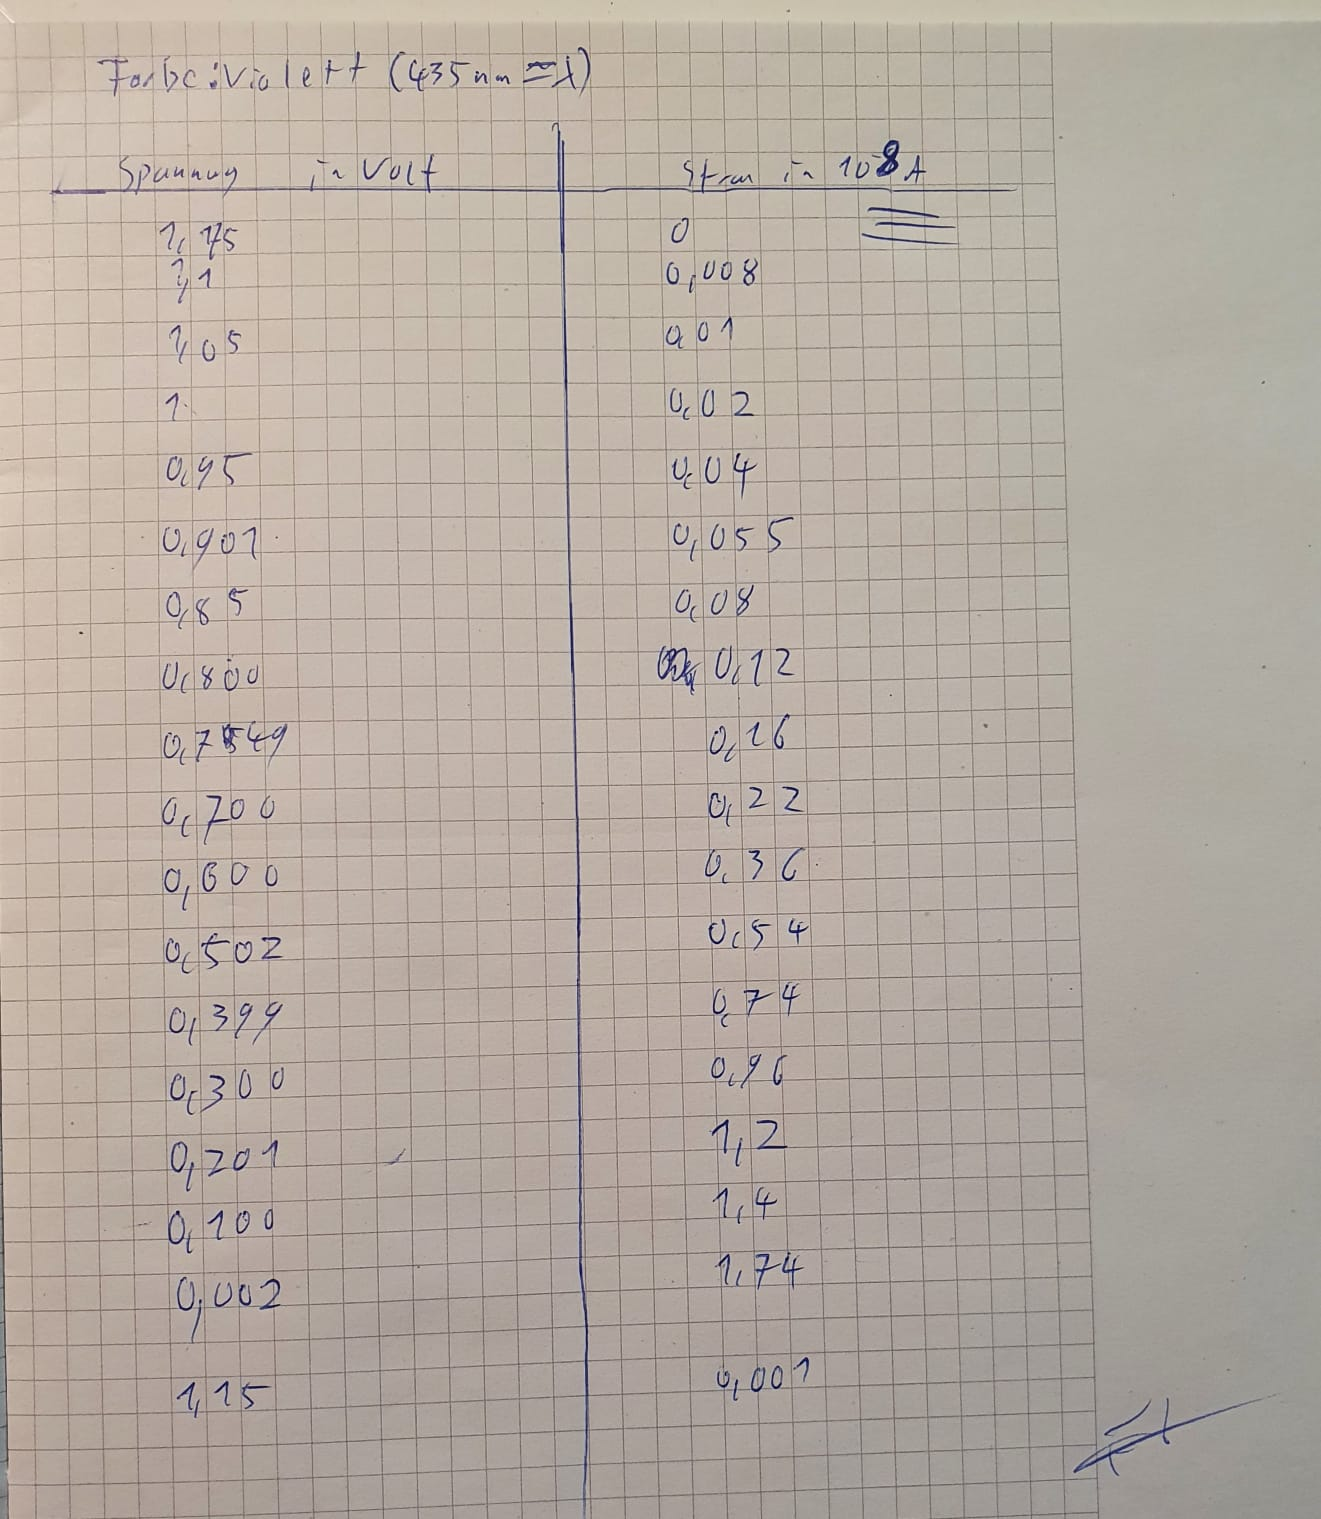
\includegraphics[width=0.63\textwidth]{latex/images/D4.jpeg}
    \caption{Ein Foto der Messdaten.}
    \label{img:Daten4}
\end{figure}

\begin{table}[H]
    \centering
    \begin{tabular}{S [table-format=2.2] S [table-format=3.2]}
        \toprule
        {$U \mathbin{\scalebox{1.5} / }\si{\volt}$} & {$I \mathbin{\scalebox{1.5} / }\si{\ampere}$}\\
        \midrule
         19.02 & 0.00\\
         15.00 & 0.00\\
         10.00 & 0.00\\
         5.00  & 0.00\\
         2.51  & 0.00\\
         0.49  & 0.02\\
         0.25  & 0.82\\
         0.15  & 1.90\\
         0.05  & 4.10\\
         0.01  & 5.20\\
        -0.05  & 6.40\\
        -0.15  & 9.50\\
        -0.25  & 12.00\\
        -0.35  & 14.50\\
        -0.50  & 16.30\\
        -0.75  & 24.00\\
        -1.00  & 29.00\\
        -1.52  & 36.00\\
        -2.50  & 51.00\\
        -5.01  & 74.00\\
        -10.01 & 94.00\\
        -15.02 & 102.00\\
        -19.12 & 105.00\\
        \bottomrule
    \end{tabular}
\caption{Die Messwerte der Messreihe vom gelben Licht.}
\label{tab:gelb}
\end{table}

\begin{table}[H]
    \centering
    \begin{tabular}{S [table-format=1.2] S [table-format=1.2]}
        \toprule
        {$U \mathbin{\scalebox{1.5} / }\si{\volt}$} & {$I \mathbin{\scalebox{1.5} / }\si{\ampere}$}\\
        \midrule
        0.55 & 0.01\\
        0.53 & 0.04\\
        0.50 & 0.08\\
        0.47 & 0.12\\
        0.45 & 0.18\\
        0.43 & 0.26\\
        0.40 & 0.35\\
        0.35 & 0.70\\
        0.30 & 1.10\\
        0.25 & 2.00\\
        0.20 & 3.05\\
        0.15 & 4.15\\
        0.10 & 5.80\\
        0.01 & 7.00\\
        0.00 & 8.50\\
        \bottomrule
    \end{tabular}
\caption{Die Messwerte der Messreihe vom grünen Licht}
\label{tab:green}
\end{table}

\begin{table}[H]
    \centering
    \begin{tabular}{S [table-format=1.2] S [table-format=1.2]}
        \toprule
        {$U \mathbin{\scalebox{1.5} / }\si{\volt}$} & {$I \mathbin{\scalebox{1.5} / }\si{\ampere}$}\\
        \midrule
        1.15 & 0.001\\
        1.10 & 0.080\\
        1.05 & 0.100\\
        1.00 & 0.200\\
        0.95 & 0.400\\
        0.90 & 0.550\\
        0.85 & 0.800\\
        0.80 & 1.200\\
        0.75 & 1.600\\
        0.70 & 2.200\\
        0.60 & 3.600\\
        0.50 & 5.400\\
        0.40 & 7.400\\
        0.30 & 9.600\\
        0.20 & 12.00\\
        0.10 & 14.00\\
        0.00 & 17.40\\
        \bottomrule
    \end{tabular}
\caption{Die Messwerte der Messreihe vom grünen Licht}
\label{tab:violett}
\end{table}

